\chapter{CERN research for exotic particles through LHC collider}
\label{chap:LHC}





Searching for exotic particles never observed before implies a need for an enormous amount of energy in the processes involved in their creation. In fact, if we want to study something never observed before at the scales of energy normally reached, it is highly unlikely we will find something new and interesting. This is the reason for which the Large Hadron Collider, briefly LHC, was designed and built.

LHC is actually the world's largest and most powerful particle accelerator. Its project was conceived in 1976 when the European particle physics community began to discuss building a Large Electron Positron (LEP) collider at CERN, and it was realized between 1998 and 2008. It required a collaboration of over 10000 scientists and hundreds of universities and laboratories, as well as more than 100 countries. It first started up on 10 September 2008, and remains the latest addition to CERN’s accelerator complex.






\section{An insight into LHC structure}
% https://home.cern/science/accelerators/large-hadron-collider
% https://home.cern/science/experiments/how-detector-works
The LHC consists of a ring 27-kilometers long of superconducting magnets with a number of accelerating structures to boost the energy of the particles along the way. Inside the accelerator, two high-energy particle beams travel at relativistic speed, close to the speed of light $c$. Before they are made to collide, they both are accelerated to a energy of the order of TeV. The two beams travel in opposite directions in separate beam pipes, which are fundamentally two tubes kept at ultrahigh vacuum. They are guided around the accelerator ring by a strong magnetic field mainteined by superconducting electromagnets, built from coils of special electric cable that operates in a superconductive state. It is of primary importance to conduct electricity with the lowest resistence, therefore loss of energy, possibile. Such technique requires cooling the magnets to a temperature close to $0~\si{K}$, which is even colder than the outer space. In order to get those temperatures, much of the accelerator is connected to a distribution system of liquid helium and the cooling phase takes a long time.

Thousands of magnets of different varieties and sizes are exploited to direct the beams around the accelerator. In total, there are\footnotemark:
\begin{itemize}
	\item 1232 dipole magnets whose length is 15 metres and their purpose is bending the beams.
	\item 392 quadrupole magnets, each 5-7 metres long, which focus the beams, thanks to their properties of magnetic lens.
\end{itemize}
\footnotetext{These technical details are taken from the official website of CERN \cite{cern}.}
Just prior to collision, another type of magnet is used to `squeeze' the particles closer together to increase the chances of collisions. In fact, the particles can be imagined as very tiny objects, so it is clear that the task of making them collide must be thought with such precision.

The beams inside LHC are made to collide at four locations around the accelerator ring, corrisponding to the positions of four particle detectors: CMS, ATLAS, ALICE and LHCb. Their placement along the collider is showed in Figure \ref{fig:LHC_COLLIDER}. All the controls for the accelerator, its services and technical infrastructure are housed at the CERN Control Centre.

\begin{figure}[t]
	\centering
	\import{Images/LHC/}{LHC_collider.tex}
	\captionof{figure}{Schematization of LHC collider.}
	\label{fig:LHC_COLLIDER}
\end{figure}





\section{CMS experiment}
% https://home.cern/science/experiments/cms
% https://cms.cern/detector
The acronym CMS means Compact Muon Solenoid and it is a general-purpose detector amongst one of the four mentioned before. It has a broad physics programme ranging from studying the Standard Model to searching for extra dimensions and particles that could make up dark matter, whose existence belongs to physics beyond the SM. CMS also stands for one of the largest international scientific collaborations in history, involving over 4000 particle physicists, engineers, technicians, students and support staff from around 200 institutes and universities from more than 40 countries.

It is built around a huge solenoid magnet. This takes the form of a cylindrical coil of superconducting cable that generates a field of 4 Tesla. The importance of this value can be better understood thinking that it is 100000 times the magnetic field of Earth. The field is confined by a steel `yoke' that forms the bulk of the detector, whose weight is about 14000 tons. It was built in 15 sections, which were reassembled in situ. The detector gets its name from the fact that:
\begin{itemize}
	\item It is 15 metres high and 21 metres long, so it is quite compact for all the detector material it contains.
	\item It is designed to detect particles known as muons (and indicated with $\mu$) very accurately.
	\item It has the most powerful solenoid magnet ever made.
\end{itemize}

\begin{figure}[t]
	\begin{center}
		\includegraphics[width=1.0\textwidth]{Images/LHC/cms.png}
		\caption{CMS detector section \cite{cms}.}
		\label{fig:CMS_SECTION}
	\end{center}
\end{figure}

The detector is shaped like a cylindrical onion, with several concentric layers of components. These components help prepare `photographs' of each collision event by determining the properties of the particles produced in that particular collision. This is done by:
\begin{itemize}
	\item \textbf{Bending particles:}\\
	A powerful magnet is needed to bend charged particles as they fly outwards from the collision point. This process is done in order to identify the charge and to measure the momentum of the particle. In fact, positive and negative charged particles bend in opposite directions in the same magnetic field and, in particular, high momentum particles bend less compared with low-momentum ones.
	
	The solenoid magnet is formed by a cylindrical coil of superconductiong fibres. A current up to $18500~\si{A}$ flows within these coils and it encounters no resistence for the phenomenon of superconductivity. The magnetic field of $4~\si{T}$ must be confined to the volume of the detector and is done by the steel `yoke' that forms the bulk of the detector's mass.
	
	\item \textbf{Identifying tracks:}\\
	It is fundamental to identify the paths taken by the bent charged particles and it must be done with extreme precision. This is done by a silicon tracker made of around 75 million individual electronic sensors arranged in concentric layers. A charged particle that passes through these layers interacts electromagnetically with the silicon and produces a signal. The information carried by individual signals can be joined together in order to identify the track of the traversing particle.
	
	\item \textbf{Measuring energy:}\\
	The energy of the various particles produced in each collision is a crucial information in the understanding of what happened in the collision process. This information is collected by calorimeters, which are particle detectors made to measure the energy. Inside CMS there are two types of these. The Electromagnetic Calorimeter (ECAL) is the inner layer of the two and measures the energy of electrons and photons by stopping them completely. The other particles, i.e. hadrons, fly through the ECAL and are stopped in the outer layer by the Hadron Calorimeter (HCAL).
	
	\item \textbf{Detecting muons:}\\
	The final particles that CMS observe directly are the muons. They are not stopped by any calorimeter, so there are other special detectors interleaved with the return yoke of the solenoid. It is possible to measure each muon's momentum both inside the superconducting coil (by the tracking devices) and outside of it (by the muon chambers).
\end{itemize}

\begin{figure}[t]
	\begin{center}
		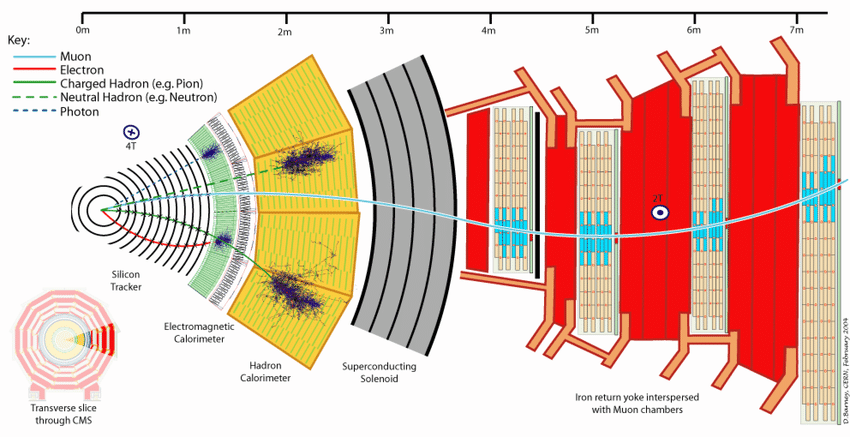
\includegraphics[width=1.0\textwidth]{Images/LHC/cms_transverse_section.png}
		\caption{CMS detector transverse section.}
		\label{fig:CMS_TRANSVERSE_SECTION}
	\end{center}
\end{figure}

Thanks to the ensemble of all these components, it is possible to detect the energies of the products of the collision, except the energies carried by neutrinos $\nu$. In fact, these are elementary particles that can't be detected by this kind of detectors. Each layer of the composition gives an information about the processes happened after the collision. By putting together all of these informations, the intermediate states of the processes could be studied as well as the laws that regulate the whole process.

As stated before, every layer can give informations about an intermediate state. So the particles observed are not the initial products of the process, but they are the traces of pre-existing unstable particles that decay in other products before the detector could observe them. The intermediate unstable states are called resonances and to better understand them it is appropriate to describe the classical definition.





\section{From data to discoveries: resonance formation study}
Resonant phenomena are ubiquitous in Physics at both the macroscopic and microscopic levels. Resonances have an extremely important role in hadron spectroscopy.

In Classical Physics, a resonance is a phenomenon that occurs when the frequency at which a periodical force is applied is equal or nearly equal to one of the natural frequencies of the system on which it acts. The visible effect of the resonance is that the system oscillates to a larger amplitude respect to the one when a force is applied with a different frequency.

The first thing to do is to analyze this phenomenon in the case of an oscillating system with an external force that drives the oscillation. The second order differential equation that describes the system is the following one:
\begin{equation}
	\devN{x}{\theta}{2} + 2 \gamma \omega_{0} \dev{x}{\theta} + \omega_{0}^2 x = \frac{F_0}{m} \sin{\Omega t} = \Gamma \sin{\Omega t}
\end{equation}
where $F_{0}$ is the amplitude of the driving force, $\Omega$ is its angular frequency, $\omega_{0}$ is the undamped angular frequency and $\gamma$ is the damping ratio. The general solution of this ODE is a combination of sinusoidal function exponentially damped and another sinusoidal function that describes a stationary state:
\begin{equation}
	x(t) = A e^{-\gamma \omega_{0}} \sin{(2\gamma \omega_{0} + \phi)} + B \sin{(\Omega t - \delta)}
\end{equation}
where:
\begin{align}
	B &= \frac{\Gamma}{\sqrt{(\omega_{0}^2 - \Omega^2)^2 + 4 \gamma^2 \omega_{0}^2 \Omega^2}}	\label{eqn:RES_B}	\\
	\delta &= \arctan{\left( \frac{2 \gamma \omega_{0} \Omega}{\omega_{0}^2 - \Omega^2} \right)}
\end{align}

The relation for the amplitude of the solution in the stationary state shows there is a maximum value for $B$, which is reached for a particular value of the angular frequency of the drive. It means that the system becomes resonant for a certain value of $\Omega$ and the transfert of energy from the drive to the system is maximized. 

Coming back to the field of subnuclear physics, a resonance appears with a shape similar to the one described by Equation \ref{eqn:RES_B}. The function describing the resonance in this case is a Breit-Wigner, reported in Equation \ref{eqn:BREIT_WIGNER}. In Figure \ref{fig:RESONANCE_PLOT} some examples are given.

\begin{equation}
	f(\mathcal{E}) \propto \frac{1}{(\mathcal{E}^2-M_{R}^2)^2 + M_{R}^2 \Gamma^2} \label{eqn:BREIT_WIGNER}
\end{equation}


\begin{figure}[H]
	\begin{center}
		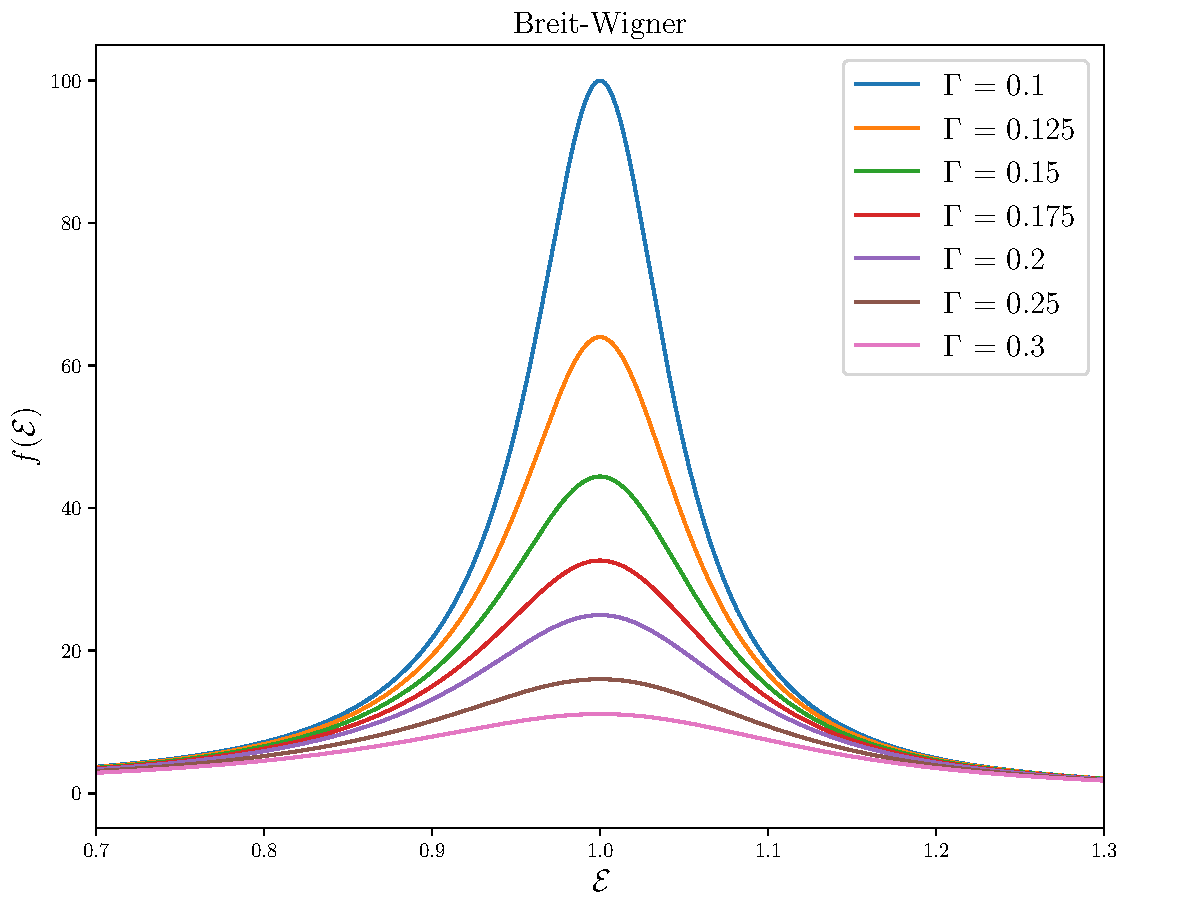
\includegraphics[width=0.4\textwidth]{Python/LHC/bw.pdf}
		\caption{Resonance plot: Breit-Wigner with $M_{R}=1$ for different choices of $\Gamma$.}
		\label{fig:RESONANCE_PLOT}
	\end{center}
\end{figure}

The extremely unstable hadrons can be observed as `resonances' in two different ways \cite{bettini}. The first approach is searching for very unstable particles by measuring as a function of energy the cross section $\sigma$ of processes of the following type:
\begin{equation}
	a + b \longrightarrow c + d + \dots + f
\end{equation}
In a quantum scattering process the relevant functions of energy are the scattering amplitude and the cross section, which is the measured observable. Near a resonance, the distribution of $\sigma$ will remark the shape of the resonant peak in Figure \ref{fig:RESONANCE_PLOT}.

\begin{figure}[H]
	\centering
	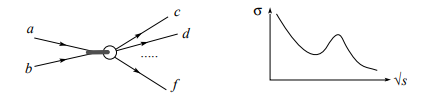
\includegraphics[width=0.7\textwidth]{Images/LHC/cross_section_resonance.PNG}
	\caption{Schematic of a resonance formation study in the cross section.}
	\label{fig:CROSS_SECTION_RESONANCE}
\end{figure}

The second approach, corresponding to a specific class of experiments, is based on resonance production. To better explain the method, let's suppose we are studying the following process:
\begin{equation}
	a + b \rightarrow c + d + e
\end{equation}
where we are searching for a particle decaying into the stable or metastable particles $c$, $d$. In this example, this particle will called $r$, which obviously stands for resonance. If $r$ exists, the decay process could develop into a second channel:
\begin{equation}
	a + b \rightarrow r + e \rightarrow c + d + e
\end{equation}
In these cases, the mass of $c+d$, called $M_{cd}$, is expected to be equal to the mass of $r$, called $M_{r}$, and it follows a Breit-Wigner distribution peaked at $M_{r}$ and with width $\Gamma$. If the decay goes directly in the final state (this is the non-resonant process), $M_{cd}$ can have any value in the range imposed by physical constraints of energy and momentum conservation, as it is a three-body decay process, and there is no peak in the distribution. Now, we have to measure the energies and the momenta for each event in order to compute:
\begin{equation}
	M_{cd} = \sqrt{(\mathcal{E}_{c} + \mathcal{E}_{d})^2 - (\vec{p}_{c} + \vec{p}_{d})^2}
\end{equation}
The resonance appears as a peak on a smooth background in the $M_{cd}$ distribution.

\begin{figure}[H]
	\centering
	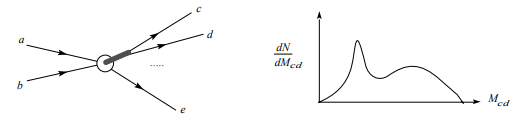
\includegraphics[width=0.7\textwidth]{Images/LHC/invariant_mass_resonance.PNG}
	\caption{Schematic of a resonance formation study in the invariant mass.}
	\label{fig:INVARIANT_MASS_RESONANCE}
\end{figure}






\begin{comment}
All the particles interact with some of the existing forces, so there exist potentials of a certain type between them, forming bound states if the energetics of the interaction are appropriate. A resonance describes a stete in these potentials that is unstable, i.e. it decays in a certain time within our observational horizon. For low, non-relativistic energies a resonance is a temporary excitation seen in scattering experiments, for example. In relativistic particle physics, particles and states are just two different languages for the same reality and so resonance could be understood as the excited level or bound state of two colliding particles.
\end{comment}